\PassOptionsToPackage{quiet}{fontspec}
\documentclass[oneside]{fduthesis2023}
\usepackage{fdumath-fduthesis-patch}
\fdusetup{
  style = {
    % fullwidth-stop    =  mapping,
    hyperlink-color   =  classic,
  },
  info = {
    author            = {无名氏},
    date / year       = { 2023 },
    student-id        = {19300180999},
    department        = {数学科学学院},
    major             = {数学与应用数学},
    supervisor        = {有名氏},
    supervisor-title  = {院士},
    supervisor-unit   = {复旦大学数学科学学院物理化学系},
    title             = {复旦大学数学科学学院本科毕业论文\LaTeX 模板(2023年版)},
    title-breakline   = {{复旦大学数学科学学院\\本科毕业论文\LaTeX 模板(2023年版)}},
    keywords          = {甲, 乙, 丙},
    keywords-english  = {A, B, C},
  },
}

\newtheorem{definition}{定义}[chapter]
\newtheorem{theorem}[definition]{定理}
\newtheorem{axiom}[definition]{公理}
\newtheorem{lemma}[definition]{引理}
\newtheorem{proposition}[definition]{命题}
\newtheorem{corollary}[definition]{推论}
\newtheorem{remark}{注}[chapter]
\def\theequation{\arabic{chapter}.\arabic{equation}}
\def\thedefinition{\arabic{chapter}.\arabic{definition}}

% \usepackage{pdfpages} % 到时候用来添加封面二和封面三
% \renewcommand{\makecoverii}{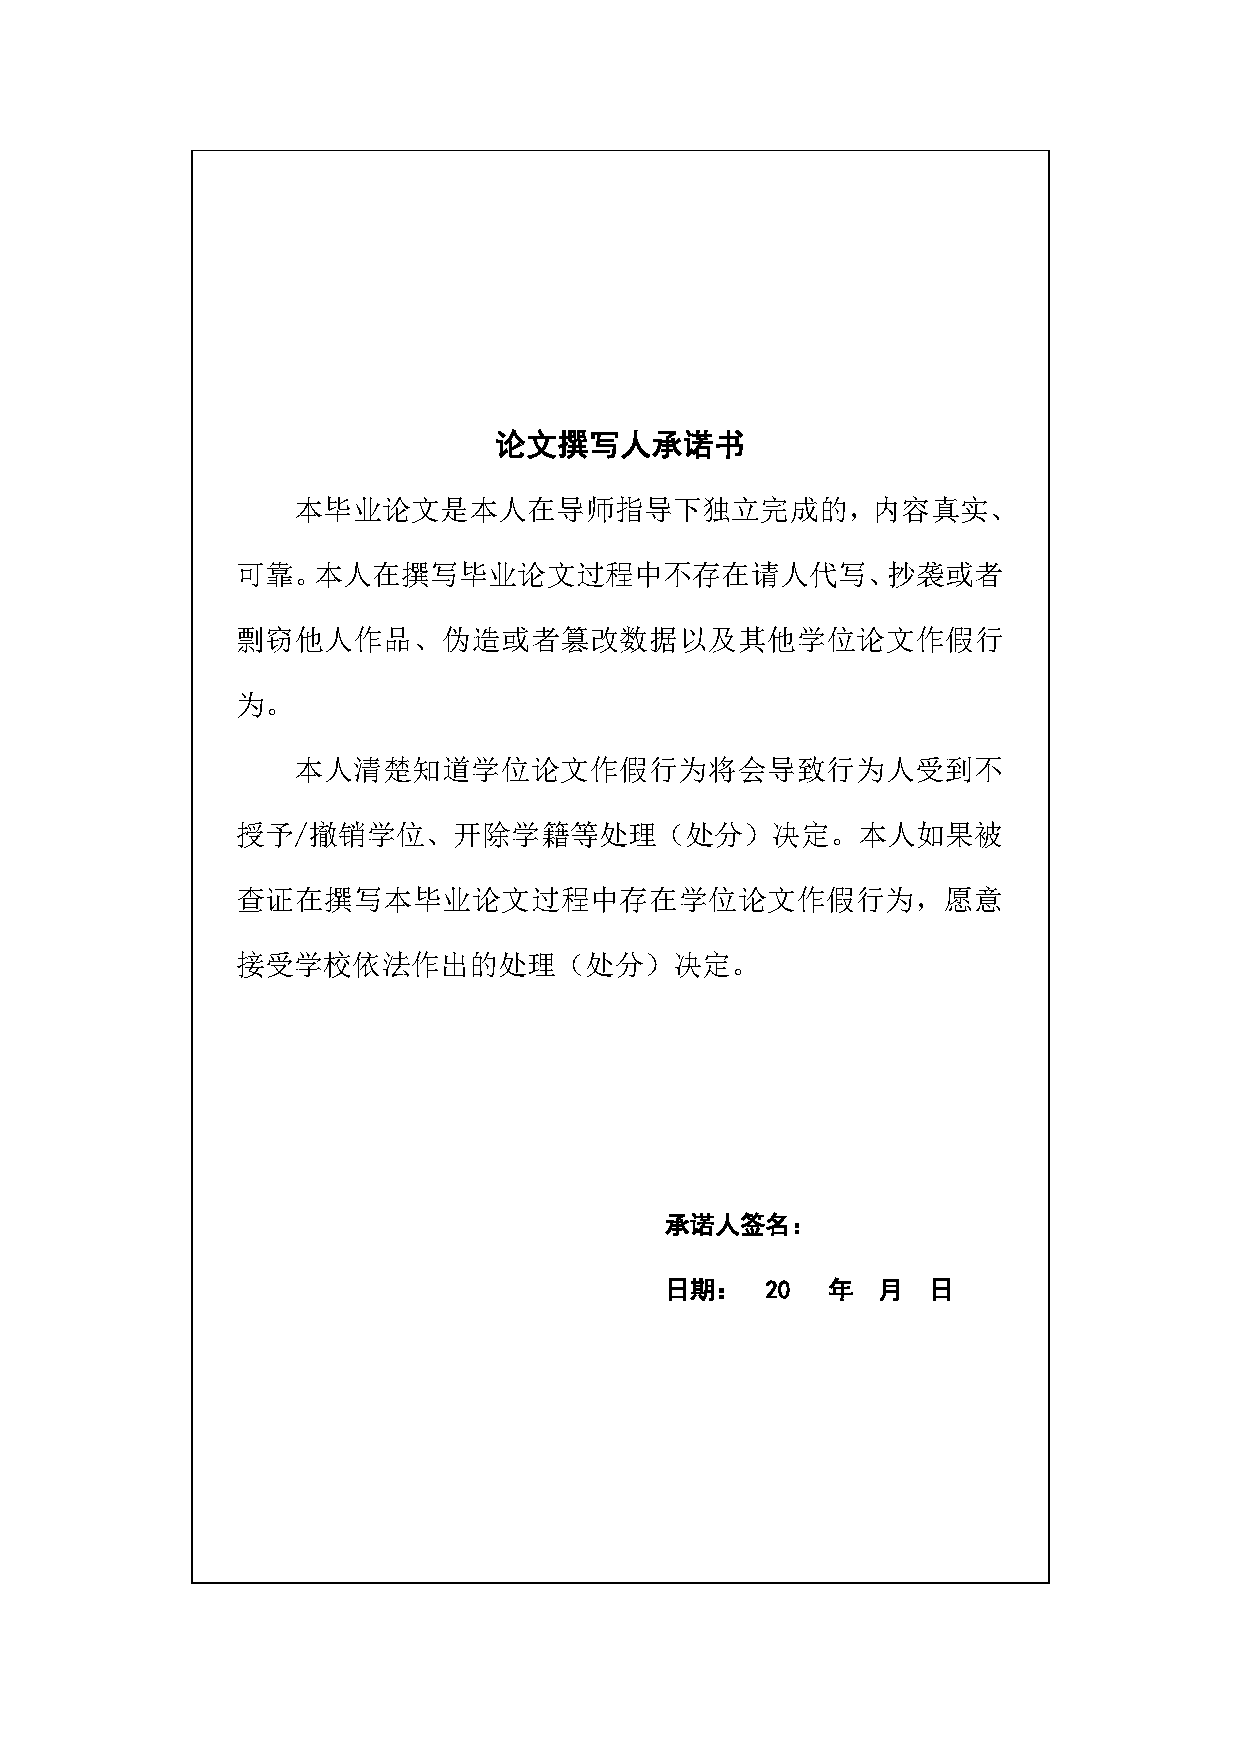
\includepdf[pages={1}]{coverii.pdf}}
% \renewcommand{\makecoveriii}{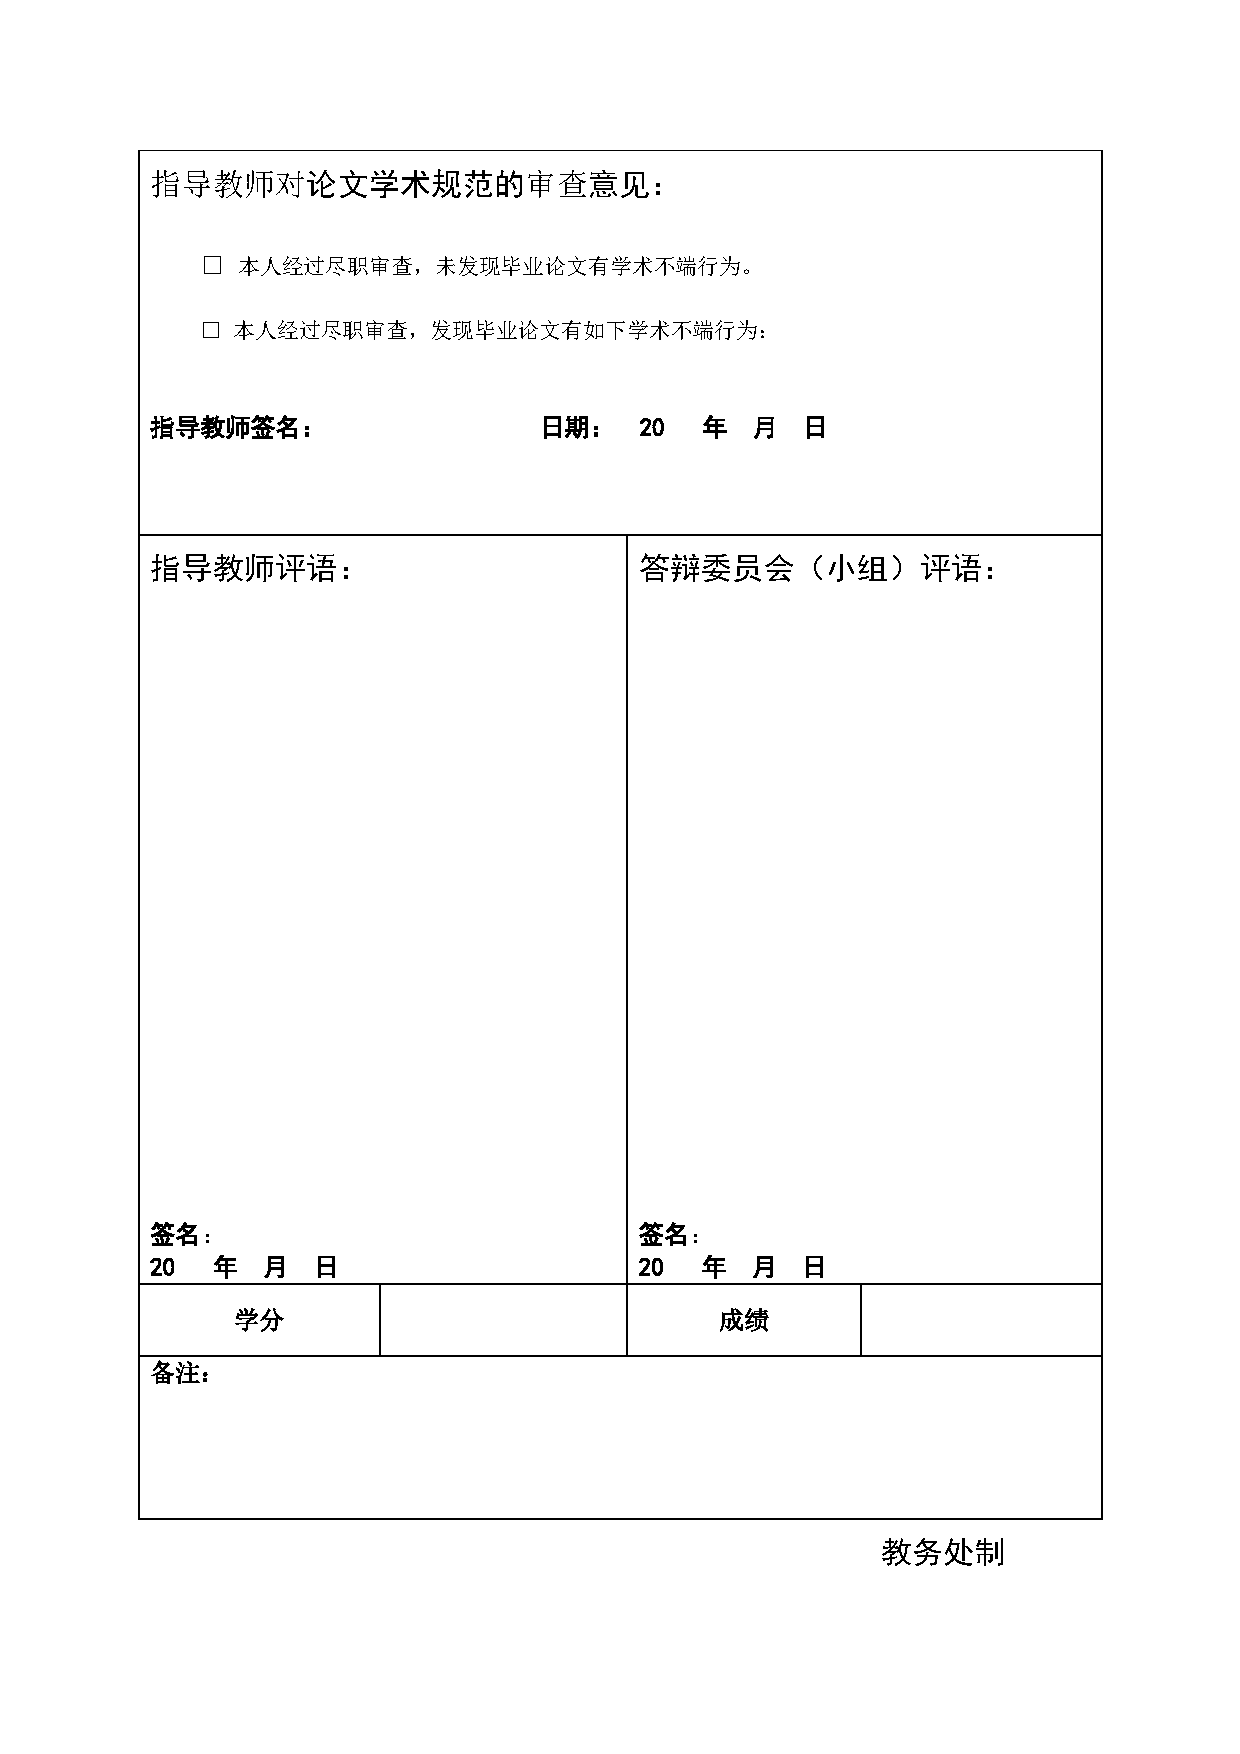
\includepdf[pages={1}]{coveriii.pdf}}

\begin{document}
  \takeCareOfPageNumbers % 修改的内容1

  \begin{abstract}
    这是摘要.
  \end{abstract}
  
  \changeToEnglishAbstract
  \begin{abstract}
    This is abstract.
  \end{abstract}

  \makeTableOfContents % 修改的内容2

  \startMainPart
  \chapter{这是章}
    \section{这是节}
      \subsection{这是小节}
        这是正文.
        $$
          f(x)=\int_{\Omega}\mathscr{A}f(g)\,\mathrm{d}\mu(\omega)
        $$
        \newpage
        这是第二页的正文.
        \begin{proof}
          Proof Ends Here.
        \end{proof}

  \backmatter
  \chapter*{致谢}
  \addcontentsline{toc}{chapter}{\textbf{致谢}}
  \renewcommand{\thepage}{}
    这是致谢.

  \clearpage
  \phantomsection\addcontentsline{toc}{chapter}{\textbf{参考文献}}
  % \bibliographystyle{unsrt}
  % \bibliography{}
\end{document} 